\subsection{Prototype}
\subsubsection{Định nghĩa}
Prototype là một loại Creational Design Pattern cho phép ta sao chép một object đã tồn tại mà không cần đoạn code ở trong chính class đối tượng đó.
\subsubsection{Cách sử dụng}
Thông thường, các trường hợp có thể sử dụng Prototype như sau:
\begin{itemize}
    \item Khi việc tạo một Object mới là một quá trình tốn kém về tài nguyên hoặc thời gian.
    \item Khi bạn muốn tránh việc chỉnh sửa mã nguồn của đối tượng gốc khi tạo ra các bản sao.
\end{itemize}
\subsubsection{Cấu trúc}
Ta có thể giải quyết vấn đề trên như sau:
\begin{itemize}
    \item 1. Tạo ra một interface hoặc abstract class có hàm clone().
    \item 2. Tạo ra một vài subclasses (Concrete Class) con kế thừa từ interface trên và implement lại hàm clone().
    \item 3. Tạo ra đối tượng bằng hàm clone().
    \item 4. Nếu cần thiết ta kết hợp cả phương pháp Factory Method, sử dụng Factory để tạo ra các đối tượng cloned một cách dễ dàng.
\end{itemize}
\begin{center}
    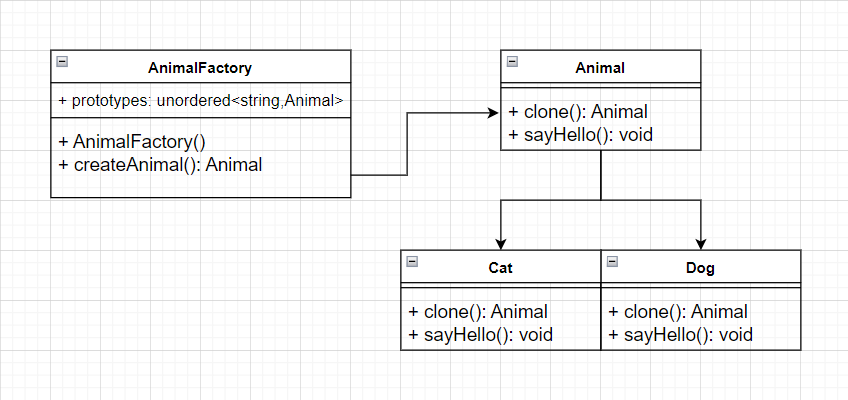
\includegraphics[scale=0.9]{image/creational/pso.png}
\end{center}
Các thành phần chính:
\begin{itemize}
    \item Một interface hay abstract class của đối tượng muốn được khởi tạo chứa hàm clone().
    \item Các Subclass kế thừa từ interface trên và có hàm clone thật chất là sử dụng copy constructor để tạo ra đối tượng mới có giá trị giống hệt đối tượng cũ.
\end{itemize}
\subsubsection{Ưu điểm và Nhược }
Ta thường thấy các ưu nhược điểm sau:\\\\
Ưu điểm:
\begin{itemize}
    \item Prototype pattern cho phép bạn tạo ra các bản sao của Object mà không cần biết lớp cụ thể của đối tượng đó. Điều này giúp giảm thiểu sự phụ thuộc và làm cho hệ thống linh hoạt hơn.
    \item Thay vì tạo ra một Object mới từ đầu, Prototype pattern cho phép sao chép các Object hiện có, giúp tiết kiệm thời gian và tài nguyên. Điều này đặc biệt hữu ích trong việc tạo ra các đối tượng phức tạp hoặc tốn kém về tài nguyên.
\end{itemize}
Nhược điểm:
\begin{itemize}
    \item  Nếu Object có các Object con hoặc liên kết với các tài nguyên khác, việc sao chép Object có thể trở nên khó khăn và mất thời gian.
    \item Đôi khi, các Object không thể hoặc không nên được sao chép. Trong trường hợp này, việc triển khai Prototype pattern có thể gặp khó khăn và không phù hợp.
\end{itemize}
\subsubsection{Code}
\begin{itemize}
    \item Ta có 2 loại động vật là chó và mèo.
    \item Một nhà máy để tạo ra một đối tượng được sao chép từ đối tượng đã được khởi tạo.
\end{itemize}
\begin{lstlisting}
#include <iostream>
#include <string>
#include <unordered_map>

using namespace std;

// Base class for prototype objects
class Animal
{
public:
    virtual Animal *clone() = 0;
    virtual void sayHello() = 0;
};

// Concrete prototype classes
class Dog : public Animal
{
public:
    Animal *clone() override { return new Dog(*this); }
    void sayHello() override { cout << "Woof!" << endl; }
};

class Cat : public Animal
{
public:
    Animal *clone() override { return new Cat(*this); }
    void sayHello() override { cout << "Meow!" << endl; }
};

// Prototype factory class
class AnimalFactory
{
public:
    AnimalFactory()
    {
        prototypes["dog"] = new Dog();
        prototypes["cat"] = new Cat();
    }

    Animal *createAnimal(string type) { return prototypes[type]->clone(); }

private:
    unordered_map<string, Animal *> prototypes;
};

int main()
{
    AnimalFactory factory;

    Animal *dog1 = factory.createAnimal("dog");
    Animal *dog2 = factory.createAnimal("dog");
    Animal *cat1 = factory.createAnimal("cat");
    Animal *cat2 = factory.createAnimal("cat");

    dog1->sayHello(); // outputs "Woof!"
    dog2->sayHello(); // outputs "Woof!"
    cat1->sayHello(); // outputs "Meow!"
    cat2->sayHello(); // outputs "Meow!"

    return 0;
} 
\end{lstlisting}
Ở hàm main, ta tạo ra đối tượng chó rồi tạo ra đối tượng được copy chó, và tương tự với đối tượng mèo.\\
\newline
\textbf{Kết quả:}
\begin{lstlisting}
Woof!
Woof!
Meow!
Meow!
\end{lstlisting}
\subsubsection{Các Pattern liên quan}
\begin{itemize}
    \item Factory và Abstract Factory ít nhiều có thể cần tạo ra các clone của nó.
    \item Commands có thể được sao lưu ở nhiều nơi.
    \item Decorator cũng có thể sử dụng để sao chép ra đối tượng mới rồi áp dụng decorator lên nó.
\end{itemize}